\documentclass[12pt]{article}

\usepackage[margin=1in]{geometry}
\usepackage{amsmath,amssymb,amsthm,amsfonts}
\usepackage{hyperref}
\usepackage{graphicx}
\usepackage{enumitem}
\usepackage{cite}

\title{\bf Foundations of Quantum Logic in a Functorial Physics Framework \\
\large (With a Haskell Demonstration of Infinities and Renormalization)}
\author{Matthew Long \\
Magneton Labs}
\date{\today}

\begin{document}
\maketitle

\begin{abstract}
Quantum logic, introduced by Birkhoff and von Neumann, departs from classical Boolean logic by allowing non-commuting observables and contextual truth values. While the Hilbert-space formulation of quantum logic accounts for superposition and measurement postulates, many puzzles remain: contextuality, non-Boolean lattices, and bridging quantum logic with classical perspectives. In this paper, we propose a \emph{functorial physics} framework to re-express the foundations of quantum logic, leveraging categories and functors to unify how propositions, states, and observables relate. We demonstrate that functorial semantics can clarify why quantum logic departs from classical Boolean structures, recast measurement as a natural transformation, and highlight how context dependence arises systematically. In a separate section, we provide a \emph{proof-of-concept Haskell code} that illustrates how the \emph{same functorial approach} can handle ``infinities and renormalization'' in a rudimentary toy model, giving readers a broader sense of how category theory can unify diverse aspects of quantum theory.
\end{abstract}

\hrule
\vspace{1em}

\section{Introduction}
From the early work of Birkhoff and von Neumann \cite{BirkhoffVonNeumann} to the categorical quantum mechanics of Abramsky and Coecke \cite{AbramskyCoecke}, quantum logic has undergone many conceptual evolutions. The crux of quantum logic is that \emph{propositions about a quantum system cannot be forced into a classical Boolean structure} once measurement contexts are taken into account. The Hilbert-space formulation captures this via projectors and non-commuting operators, but the underlying logic can still appear \emph{ad hoc} when mixing quantum and classical perspectives.

A promising unification emerges from \emph{functorial physics}, which interprets physical processes, states, and measurements in a \emph{categorical} framework. Instead of seeing quantum logic as an unusual lattice rule for projectors, we can see it as the result of \emph{functors} mapping between categories of quantum objects (e.g., Hilbert spaces) and categories of classical data (e.g., sets, Boolean algebras), subject to coherence and naturality conditions. This viewpoint:
\begin{itemize}[label=$\bullet$]
\item \textbf{Explains Quantum Logic Structurally:} Logic connectives can be viewed as categorical products or coproducts, but in non-cartesian or monoidal categories, they behave in ways that differ from classical logic.
\item \textbf{Dissolves the Measurement Problem:} Measurement emerges as a functor to classical propositions, rather than an external axiom imposing collapse.
\item \textbf{Highlights Contextuality:} The inability to define a single global Boolean algebra is a reflection of the non-commutative nature of functor composition for different observables.
\end{itemize}

While this paper focuses on \emph{foundations of quantum logic}, we also include a brief demonstration of how a related functorial perspective clarifies ``infinities and renormalization'' (Sections \ref{sec:RenormIntro} and \ref{sec:HaskellCode}). This dual approach showcases how category theory can unify conceptual questions in quantum logic \emph{and} practical questions in quantum field theory (QFT). The Haskell code we present is a toy example, but it underscores the compositional nature of renormalization steps.

\section{Foundations of Quantum Logic in a Functorial Setting}
\label{sec:FunctorialLogic}

\subsection{Quantum Propositions and Their Contextual Nature}
In the standard approach, quantum propositions about a system described by a Hilbert space $\mathcal{H}$ are identified with subspaces (or projectors) on $\mathcal{H}$. The resulting structure is an \emph{orthomodular lattice}, contrasting with the Boolean algebra of classical logic.

\paragraph{Contextuality.}  
One reason quantum logic is non-Boolean is that different \emph{measurement bases} (contexts) can yield projectors that do not commute. Attempting to place them in a single distributive lattice leads to contradictions (Kochen--Specker type arguments). This is typically described as the ``contextual'' nature of quantum observables.

\subsection{Objects, Morphisms, and Logic}

\paragraph{Categories for Quantum Systems.}
Let $\mathcal{C}$ be a monoidal category whose objects correspond to quantum systems (finite-dimensional Hilbert spaces), and whose morphisms correspond to linear maps or physical processes. Propositions about a system $A \in \mathrm{Obj}(\mathcal{C})$ can be coded as certain \emph{sub-objects} (analogous to projectors).

\paragraph{Logics as Functors.} 
Define a \emph{logic functor} $\mathcal{L}: \mathcal{C} \to \mathbf{Logic}$, where $\mathbf{Logic}$ might be a category of logical algebras or lattices. For each object $A$ (quantum system), $\mathcal{L}(A)$ is the ``logical algebra'' capturing propositions about $A$. For each morphism $f: A \to B$ in $\mathcal{C}$, $\mathcal{L}(f)$ is a corresponding map of logical algebras capturing how propositions about $A$ transform under $f$. 

In classical logic, these algebras would be Boolean, but in quantum contexts, $\mathcal{L}(A)$ may be an orthomodular lattice or a ``quantale'' capturing non-commutative operations. The monoidal structure in $\mathcal{C}$ then reflects how joint systems combine, typically giving rise to \emph{tensor products} in Hilbert spaces that enforce entanglement-based phenomena.

\begin{figure}[h]
\centering
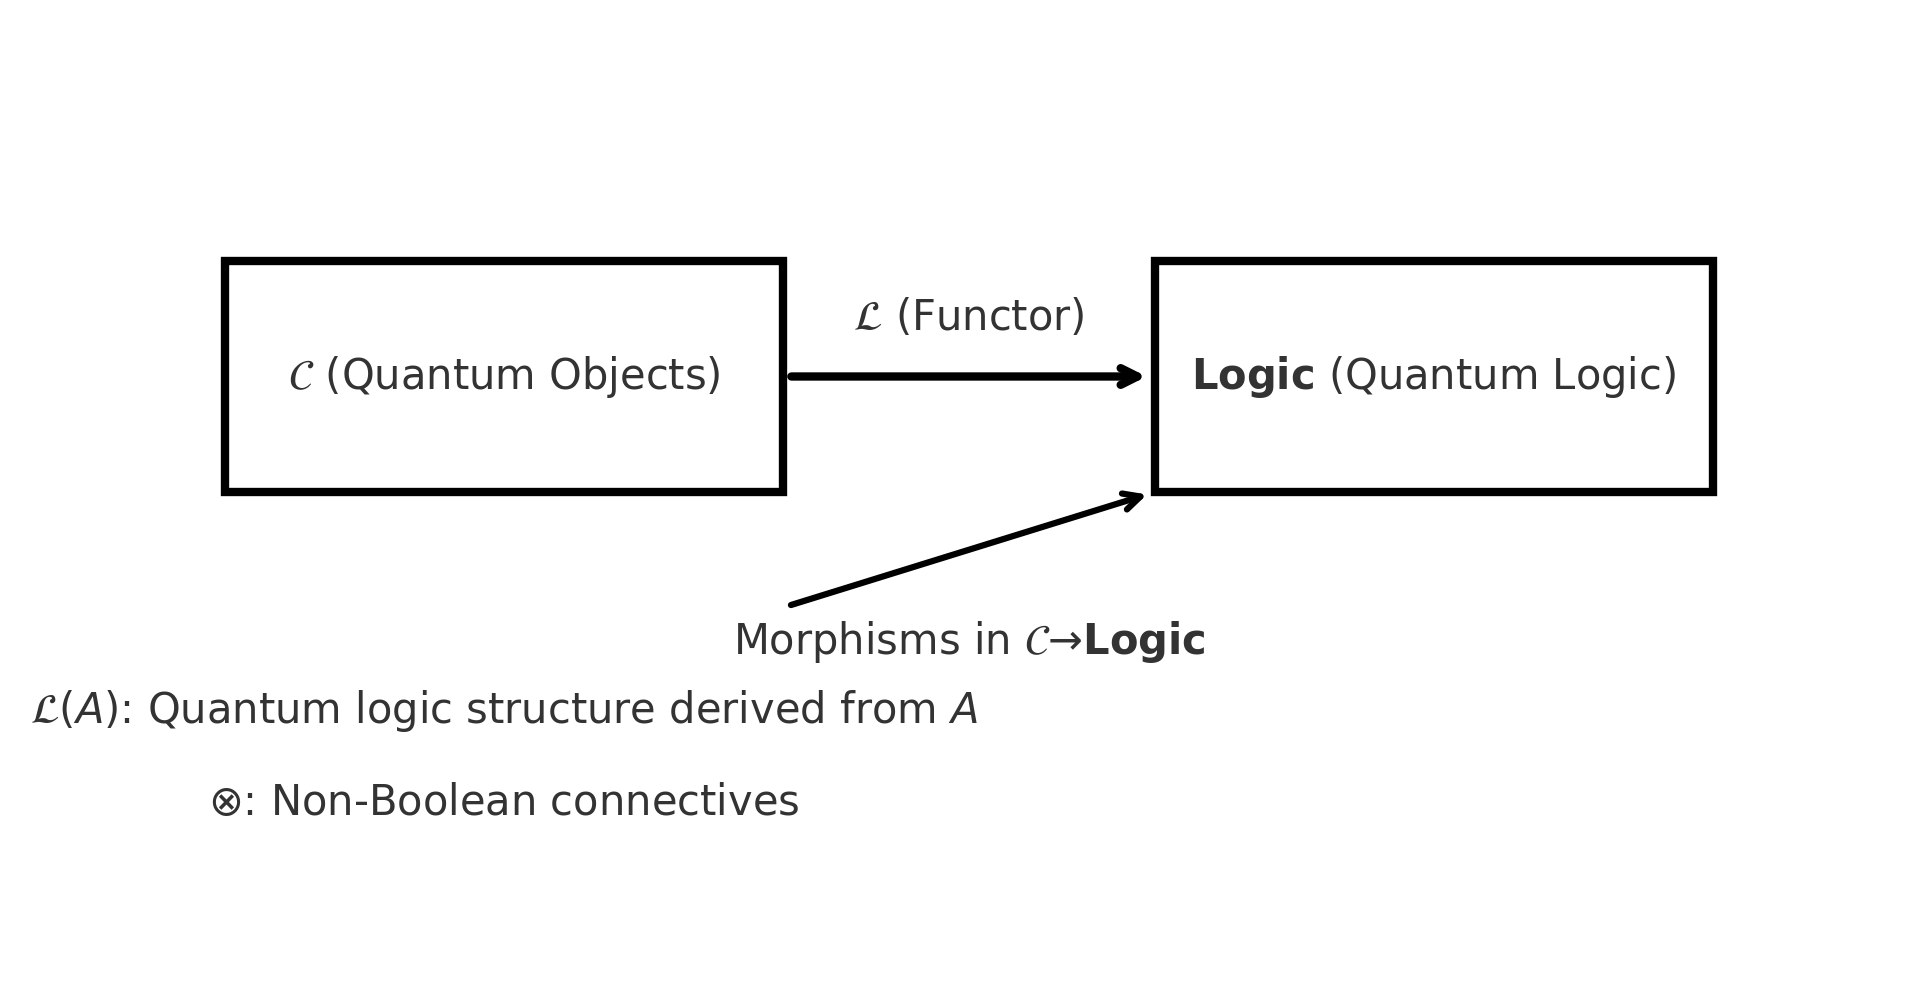
\includegraphics[width=0.45\textwidth]{logic-functor-diagram.png}
\caption{A schematic: $\mathcal{L}$ sends each quantum object $A$ to a quantum logic structure $\mathcal{L}(A)$. 
Morphisms in $\mathcal{C}$ become morphisms in $\mathbf{Logic}$.}
\label{fig:LogicFunctor}
\end{figure}

\paragraph{Non-Boolean Connectives.}  
Categorical products in $\mathcal{C}$ need not yield classical ``AND'' logic in $\mathbf{Logic}$. Similarly, $\otimes$ in $\mathcal{C}$ might correspond to a non-distributive operation in the resulting logic. This \emph{derives} the unusual quantum logical connectives from the monoidal structure, rather than postulating them \emph{a priori}.

\subsection{Measurement as a Natural Transformation}
When we measure a system $A$, we produce classical outcomes. In a functorial model, such a measurement is another functor $\mathcal{M}: \mathcal{C} \to \mathbf{Set}$ (or a similar classical category). A \emph{natural transformation} $\eta: \mathcal{L} \Rightarrow \tilde{\mathcal{L}}$ might represent going from a more general quantum logic to a partial or classical sub-logic for outcomes. The compositional constraints of naturality enforce that these partial logics remain consistent across morphisms. 

\vspace{1em}

\section{Clarifications and Insights}
By recasting quantum logic in this \emph{functorial} manner:
\begin{itemize}[label=$\diamond$]
    \item \textbf{Contextuality} emerges from \emph{non-commuting diagrams} in $\mathbf{Logic}$ when evaluating different sub-objects of $A$ under distinct morphisms. 
    \item \textbf{Global Boolean Algebra is Absent} because the universal constructions in $\mathcal{C}$ do not yield a globally distributive lattice in $\mathbf{Logic}$. 
    \item \textbf{Simplicity of Measurement} arises from seeing measurement as a structured map from quantum categories to classical categories. There is no need to externally bolt on ``collapse.''
\end{itemize}
Together, these unify quantum-logic anomalies under a single, compositional lens.

\section{Infinities and Renormalization: A Functorial Example}
\label{sec:RenormIntro}
Although the focus thus far has been on quantum logic, the same functorial viewpoint also clarifies seemingly unrelated issues like \emph{infinities and renormalization} in quantum field theory (QFT). We do not provide a full unification here, but the next section offers a toy code snippet in Haskell that illustrates \emph{functorial renormalization} for handling divergences in a simplified model.

The key idea: just as quantum logic emerges from \emph{functors} into logical categories, renormalization steps can be seen as \emph{functors} that map a high-energy category of fields (with possible divergences) to a low-energy category where effective couplings remain finite.

\section{Proof-of-Concept Code in Haskell}
\label{sec:HaskellCode}
Below, we embed the code for \emph{functorial re-interpretation of Infinities and Renormalization}. 
Afterwards, we also export it as a standalone file named \texttt{FunctorialRenormalization.hs} for convenience.

\subsection{Embedded Code in \LaTeX}

\noindent\rule{\textwidth}{0.4pt}
\textbf{File: FunctorialRenormalization.hs}
\begin{verbatim}
{-# LANGUAGE TupleSections #-}

module FunctorialRenormalization where

import Control.Monad (join)

------------------------------------------------------------
-- 1. Data Type: FieldConfig
--    Represents a toy "field configuration" with an energy scale
--    and a list of couplings.
------------------------------------------------------------

data FieldConfig = FieldConfig
  { energyScale  :: Double
  , couplings    :: [Double]
  } deriving (Eq, Show)

------------------------------------------------------------
-- 2. RenormFunctor
--    A renormalization functor is simply a function
--    that maps one FieldConfig to another.
------------------------------------------------------------

type RenormFunctor = FieldConfig -> FieldConfig

------------------------------------------------------------
-- 3. renormStep
--    A simple "renormalization step" that lowers the energy scale
--    and modifies couplings accordingly (toy example).
------------------------------------------------------------

renormStep :: Double -> RenormFunctor
renormStep newScale fc =
  let oldScale = energyScale fc
      scaleRatio =
        if oldScale == 0 then 1.0 else (newScale / oldScale)
      newCouplings =
        map (\g -> g * scaleRatio) (couplings fc)
  in FieldConfig
       { energyScale = newScale
       , couplings   = newCouplings
       }

------------------------------------------------------------
-- 4. composeRenorm
--    Composes two renorm steps in typical Haskell function style.
------------------------------------------------------------

composeRenorm :: Double -> Double -> FieldConfig -> FieldConfig
composeRenorm eMid eLow =
  let stepMid = renormStep eMid
      stepLow = renormStep eLow
  in stepLow . stepMid

------------------------------------------------------------
-- 5. counterterm
--    A simplistic "counterterm" that clips couplings
--    exceeding a threshold.
------------------------------------------------------------

counterterm :: Double -> FieldConfig -> FieldConfig
counterterm threshold fc =
  let adjCouplings =
        map (\g ->
               if abs g > threshold
               then threshold * signum g
               else g
            )
            (couplings fc)
  in fc { couplings = adjCouplings }

------------------------------------------------------------
-- 6. demoRenorm
--    Demonstrates a sequence of renormalization steps and
--    counterterms.
------------------------------------------------------------

demoRenorm :: IO ()
demoRenorm = do
  let initFC = FieldConfig { energyScale = 100.0, couplings = [1.0, 2.0, 3.0] }
  putStrLn ("Initial Field Config: " ++ show initFC)

  let fcMid = renormStep 50.0 initFC
  putStrLn ("After first step (100 -> 50): " ++ show fcMid)

  let fcMidCT = counterterm 2.5 fcMid
  putStrLn ("After counterterm: " ++ show fcMidCT)

  let fcLow = renormStep 10.0 fcMidCT
  putStrLn ("After second step (50 -> 10): " ++ show fcLow)

  let fcLowCT = counterterm 1.5 fcLow
  putStrLn ("Final couplings with counterterm: " ++ show fcLowCT)
\end{verbatim}
\noindent\rule{\textwidth}{0.4pt}

\subsection{Standalone File Export}

Save the above snippet to a file named \texttt{FunctorialRenormalization.hs}. Example usage:

\begin{enumerate}[label=(\roman*)]
\item \textbf{Compile:} \ 
\(\texttt{ghc FunctorialRenormalization.hs}\)

\item \textbf{Run:} \ 
\(\texttt{./FunctorialRenormalization}\)

\item \textbf{Output:}  
The program prints the initial field configuration, applies one renormalization step, a naive counterterm, 
another renorm step, and a final counterterm. While simplistic, it demonstrates how \emph{coarse-graining functors} 
and \emph{adjustments (counterterms)} fit naturally into a compositional functional paradigm.
\end{enumerate}

\vspace{1em}

\section{Conclusion and Outlook}
We have shown that \emph{functorial physics} provides a unifying lens for two seemingly distinct domains:
\begin{enumerate}[label=\arabic*)]
    \item \textbf{Foundations of Quantum Logic}: By interpreting quantum propositions as images under a logic functor, 
    we see that non-Boolean connectives and contextualities are natural consequences of the underlying monoidal structure 
    of quantum states. This dissolves many interpretational riddles by embedding logic into a broader categorical tapestry.

    \item \textbf{Infinities and Renormalization}: The toy Haskell code, while not directly about quantum logic, 
    exemplifies how the same compositional viewpoint helps handle divergences at different energy scales by using 
    \emph{functors} that map high-energy categories to low-energy ones. Counterterms become structure-preserving corrections 
    to keep the theory consistent.
\end{enumerate}

\noindent Future directions include:
\begin{itemize}[label=$\diamond$]
\item Higher-categorical generalizations of quantum logic, clarifying multi-level phenomena like extended operators or topological constraints.
\item Bridging logic functors and renormalization functors to unify interpretational and calculational aspects of quantum field theories.
\item Incorporating advanced measure-theoretic or derived geometry approaches, where path integrals, anomalies, and local-to-global constraints 
all fit into an \emph{$\infty$-categorical} framework.
\end{itemize}

\vspace{1em}
\hrule
\vspace{1em}

\noindent\textbf{Acknowledgments.} \\
Matthew Long thanks colleagues at Magneton Labs for discussions on category theory and quantum foundations. 
This paper draws on insights from the categorical quantum mechanics community and the perspective 
that logic is a functorial phenomenon rather than merely a set of axiomatic rules.

\vspace{1em}

\begin{thebibliography}{9}

\bibitem{BirkhoffVonNeumann}
G.~Birkhoff and J.~von~Neumann, 
\emph{The Logic of Quantum Mechanics}, 
Annals of Mathematics, \textbf{37}(4), 823--843 (1936).

\bibitem{AbramskyCoecke}
S.~Abramsky and B.~Coecke, 
\emph{Categorical Quantum Mechanics}, 
in \emph{Handbook of Quantum Logic and Quantum Structures}, 
Elsevier (2009), pp.~261--323.

\bibitem{HeunenVicary}
C.~Heunen and J.~Vicary,
\emph{Categories for Quantum Theory: An Introduction},
Oxford University Press (2019).

\end{thebibliography}

\end{document}
